\section{Progettazione}
\todo{Aggiungere UML, UseCases diagram e template, MockUps, Navigation Diagram ed ER? meglio dire come gestiamo il database in memoria e jpa/hibernate}
\todo[color=blue]{Andre scrivi il paragrafo 3 sul database ovvero parla di hibernate,transaction manager e come hai annotato le clsse e del
    database in memoria}

\subsection{JPA}
vantaggi nell'uso di JPA:
\begin{enumerate}
    \item \textbf{Possesso della persistenza nel codice} \newline
          Come è noto, le annotazioni JPA definiscono lo schema logico della persistence unit
          assunto dall'applicazione, nel contesto più generale in cui la persistence unit ha
          esistenza autonoma ed è condivisa con una pluralità di attori.
          Di conseguenza, non è richiesto che tali assunzioni rispecchino le reali proprietà
          della persistence unit, ma soltanto che siano covarianti rispetto ad esse:
          ad esempio, contemplando un sottoinsieme delle tabelle o l'esistenza di vincoli più stringenti.

          Nel nostro caso tuttavia la persistence unit non era preesistente e autonoma
          rispetto all'applicazione, anzi avremmo dovuto progettarla insieme all'applicazione stessa:
          in questo contesto, utilizzare JPA ci è sembrato particolarmente utile in quanto ci consentiva,
          attraverso opzioni di bootstrap vendor-specific - per Hibernate, la bootstrap property
          \texttt{hibernate.hbm2ddl.auto = create-drop} - di imporre al database esattamente
          lo schema fisico determinato dalle annotazioni JPA.

          Questo però non garantiva pienamente l'inversione della dipendenza, in quanto
          restavano dipendenti dallo schema fisico alcune porzioni critiche di codice: ad esempio,
          le annotazioni @UniqueConstraint() che definisce vincoli di unicità, @MappedBy() che stabilisce
          la owning side di un attributo collettivo, e soprattutto la logica di query.
          Per garantire la code ownership ci siamo serviti di un ulteriore strumento JPA,
          il JPA Metamodel Generator: un annotation processor che produce automaticamente
          in fase di compilazione classi contenenti i dettagli fisici delle tabelle desunte
          dalle annotazioni.

          In questo modo, abbiamo finalmente raggiunto l'obettivo della dependency inversion
          fra codice e persistenza: non è la persistenza ad obbligare il codice a conformarsi
          ad essa, ma il codice che possiede la specifica delle proprietà della persistenza.

          Questa inversione porta i seguenti vantaggi:
          \begin{itemize}
              \item lo schema fisico della persistence unit non è minimamente di intralcio 
                    all'evoluzione della modellazione del dominio, in quanto è automaticamente 
                    inferito da questa in fase di esecuzione
              \item la modellazione del dominio può essere quindi rivista e modificata con la
                    velocità di evoluzone di un tipo Java, incoraggiando la ricerca di
                    soluzioni efficaci per il gli attori del sistema
          \end{itemize}

    \item \textbf{Object-relational mapping} \newline
          JPA ci ha permesso di non dover gestire il flusso di informazione dalla JVM al database e viceversa,
          che altrimenti andrebbe implementato manualmente in JDBC. Sono sufficienti le mapping annotations
          e le convenzioni JPA
    \item \textbf{Transazionalità} \newline
          Un ulteriore vantaggio derivato dall'uso di JPA è la possibilità di rendere una unit of work
          transazionale
\end{enumerate}

Di seguito descriviamo alcuni aspetti notevoli del nostro uso di JPA.

\begin{itemize}
    \item \textbf{rispetto del layering} \newline
        Per quanto JPA sia una tecnologia robusta e sicura, ci è comunque sembrato opportuno
        progettare i core layers in maniera da non dipendere da alcun dettaglio implementativo: 
        l'uso di una dterminata tecnologia di gestione della persistenza come JPA, di uno specifico 
        vendor JPA come Hibernate, o peggio ancora di uno specifico DBMS come Postgres. 

        \textit{JPA-agnosticism nella Business Logic} \newline
        i Services che compongono la Business Logic non dipendono dalla presenza di JPA, in quanto
        \begin{itemize}
              \item definiscono interfacce per le "collezioni di entità di un certo tipo presenti
                    nel sistema", ovvero vari EntityRepository, ed una denominata TransactionManager
                    che espone API per l'esecuzione transazionale di una unit-of-work sui Repositories
              \item vengono istanziati su una istanza di TransactionManager e si servono delle sue API
                    per eseguire operazioni sui dati presenti nel sistema in maniera transazionale
        \end{itemize}
        A runtime, i Services riceveranno un implementatore concreto di TransactionManager: 
        tuttavia, il codice dei Services è del tutto privo di assunzioni sulla tecnologia 
        effettivamente utilizzata per implementarlo.

        \textit{Hibernate-agnosticism nel Data-Access Layer} \newline
        i Repositories e TransactionManager concreti dipendono solo da JPA, in quanto
        \begin{itemize}
              \item i JpaEntityRepositories richiedono di essere istanziati su un EntityManager JPA,
                    e di esso si servono per eseguire operazioni sulla collezione
                    delle entità di cui sono responsabili o di entità associate. Tuttavia, tali
                    queries sono formulate in un DDL vendor-agnostic (Jpa Criteria Queries) 
                    e non uno vendor-specific come Hibernate Query Language
              \item JpaTransactionManager implementa TransactionManager in termini di 
                    EntityManager.beginTransaction() etc. e istanziando i JpaEntityRepositories
        \end{itemize}
        In questo modo, i JpaEntityRepositories e JpaTransactionManager non fanno assunzioni 
        sul vendor JPA effettivamente utilizzato, e sono quindi riusabili in presenza di 
        un qualsiasi vendor JPA diverso da Hibernate.

    \item \textbf{qualità delle astrazioni nel domain modelling} \newline
        Nel fare modellazione del dominio ci siamo spesso chiesti se la forma naturalmente suggerita 
        dal modello relazionale ad un dato ambito del dominio fosse realmente la più intuitiva 
        per i componenti applicativi del sistema. Ad esempio, il modello relazionale impone che 
        la relazione molti-a-molti fra Team e Player venga reificata, attraverso una ulteriore 
        entità che potremmo chiamare "Contract". Tuttavia, il codice applicativo non ha beneficio 
        nel rapportarsi con il tipo Contract; semmai, vorrebbe vedere un Team come l'insieme dei 
        suoi Player, ovvero accedere alla composizione di un Team tramite una API simile a 
        Team.getGoalkeepers().
        Le soluzioni che abbiamo adottato, basate @MappedBy con attributi collettivi e l'uso 
        di fluent APIs, cercano di fornire al codice applicativo una visione del dominio 
        idiomatica e libera dalle imposizioni della persistenza relazionale.

    \item \textbf{rappresentazione dell'informazione di tipo} \newline
        Nel modellare il dominio, ci siamo posti il problema di come rappresentare l'informazione
        di tipo nelle entità: ad esempio, il fatto che un Player ha un ruolo, o che una LineUp
        contiene un determinato modulo. Le soluzioni che abbiamo adottato sono state due:
         \begin{itemize}
              \item Entity Inheritance quando l'informazione di tipo è connaturata all'entità, 
                    ovvero non muta durante il ciclo di vita di una occorrenza di tale entità:
                    è il caso del ruolo di un giocatore, per cui Goalkeeper e Defender sono
                    entity-subtypes di Player. Ci siamo poi dovuti avvalere del pattern Visitor
                    per implementare logica che discrimina sul tipo runtime, a causa di una
                    limitazione imposta da Hibernate per cui le entità non possono essere
                    classi sealed
              \item type-mapping quando l'informazione di tipo è mutevole nel ciclo di vita
                    di una occorrenza. In questo caso, ci siamo serviti degli Enum con controllo
                    di esaustività presenti in Java 14+ come nel caso di MatchDay, 
                    oppure di soluzioni ibride come per LineUp: il tipo Scheme, che rappresenta 
                    il modulo calcistico
                    utilizzato nella formazione, è un tipo Java ma realizza di fatto la semantica di
                    un Enum. I suoi sottotipi concreti, come gli schemi "4-3-3" e "3-4-3", vengono generati
                    automaticamente da un annotation processor. Un vantaggio di questa soluzione 
                    apparentemente scomoda è
                    che i componenti dipendenti da Scheme non sono costretti a cononscere
                    le varianti concrete di schema effettivamente presenti nel sistema
        \end{itemize}

    \item \textbf{lazy fetching nelle entità, deep fetching nel DAL} \newline
        Dal momento che la nostra logica di accesso al dato non si avvantaggiava mai 
        del lazy fetching offerto da EntityManager, avremmo potuto forzare il fetching 
        a eager direttamente dalle annotazioni di associazione nelle entità. Invece, 
        abbiamo preferito seguire il suggerimento del manuale Hibernate e non imporre una 
        fetching policy a livello di associazione, in modo da lasciare libertà alla 
        data access logic di specificare la propria. In questo modo, le nostre entità 
        risultano riusabili anche in presenza di un Data Access layer radicalmente diverso

\end{itemize}


\todo[color=green]{Nicco crea gli use case template scegline qualcuno che ritieni significativo NON login e register}

\subsection{Use Case Templates}

\begin{table}[H]
\caption{Crea fantalega}
\label{UC-01}

\begin{tabularx}{\textwidth}{|l|X|}
\hline
\textbf{Id} & UC-01 (Crea fantalega) \\
\hline
\textbf{Scope} & user goal \\
\hline
\textbf{Descrizione} & L'utente vuole creare una nuova fantalega di cui sarà admin. \\
\hline
\textbf{Attori} & Admin \\
\hline
\textbf{Flusso base} &
\begin{enumerate}[leftmargin=*]
    \item L'utente inserisce il nome e il codice della lega che vuole creare.
    \item Il sistema verifica che non sia già presente una lega con lo stesso codice.
    \item Se i dati sono validi, il sistema crea la nuova lega.
\end{enumerate} \\
\hline
\textbf{Flusso alternativo} &
\begin{enumerate}[leftmargin=*,label=2.\arabic*]
    \item Il codice scelto è già utilizzato per un'altra lega.
    \item Il sistema mostra a schermo un messaggio di errore, specificando la causa del problema.
\end{enumerate} \\
\hline
\textbf{Test} & \hyperref[IT3]{IT3} \\
\hline
\end{tabularx}

\end{table}



\begin{table}[H]
\caption{Assegna giocatori alle rose}
\label{UC-02}

\begin{tabularx}{\textwidth}{|l|X|}
\hline
\textbf{Id} & UC-02 (Assegna giocatori alle rose) \\
\hline
\textbf{Scope} & user goal \\
\hline
\textbf{Descrizione} & L'admin vuole assegnare i giocatori corretti alle rose presenti nella lega. \\
\hline
\textbf{Attori} & Admin \\
\hline
\textbf{Flusso base} &
\begin{enumerate}[leftmargin=*]
    \item L'admin inserisce il team e il giocatore che deve essere assegnato a tale team.
    \item Il sistema verifica che il numero massimo di giocatori nel team non sia già stato raggiunto.
    \item Il sistema verifica che il numero massimo di giocatori nel team appartenenti allo 
            stesso ruolo del nuovo giocatore non sia già stato raggiunto.
    \item Il sistema salva il nuovo contratto tra team e giocatore.
\end{enumerate} \\
\hline
\textbf{Flusso alternativo} &
\begin{enumerate}[leftmargin=*,label=2.\arabic*]
    \item Il numero massimo di giocatori nel team è già stato raggiunto.
    \item Il sistema mostra a schermo un messaggio di errore, specificando la causa del problema.
\end{enumerate}
\begin{enumerate}[leftmargin=*,label=3.\arabic*]
    \item Il numero massimo di giocatori nel team appartenenti allo stesso ruolo
            del nuovo giocatore è già stato raggiunto.
    \item Il sistema mostra a schermo un messaggio di errore, specificando la causa del problema.
\end{enumerate} \\
\hline
\textbf{Test} & \hyperref[IT5]{IT5} \\
\hline
\end{tabularx}

\end{table}



\begin{table}[H]
\caption{Inserisci formazione}
\label{UC-03}

\begin{tabularx}{\textwidth}{|l|X|}
\hline
\textbf{Id} & UC-03 (Inserisci formazione) \\
\hline
\textbf{Scope} & user goal \\
\hline
\textbf{Descrizione} & L'utente vuole inserire la formazione per giocare la partita successiva. \\
\hline
\textbf{Attori} & FantaUser \\
\hline
\textbf{Flusso base} &
\begin{enumerate}[leftmargin=*]
    \item L'utente fornisce la LineUp che vuole utilizzare per la partita successiva.
    \item Il sistema verifica che la data in cui viene effettuata l'operazione 
            sia precedente alla data della partita.
    \item Il sistema verifica che la data in cui viene effettuata l'operazione 
            non sia un sabato o una domenica.
    \item Se la partita non è la prima del campionato, il sistema verifica che 
            i voti per la partita precedente siano già stati calcolati. 
    \item Il sistema verifica che i giocatori appartenenti alla formazione 
            siano giocatori posseduti dall'utente.
    \item Se l'utente ha già stata inserito una formazione per la partita, 
            il sistema la elimina per poter inserire la nuova formazione.
    \item Il sistema salva la formazione per la partita successiva.
\end{enumerate} \\
\hline
\textbf{Flusso alternativo} &
\begin{enumerate}[leftmargin=*,label=2.\arabic*]
    \item La data in cui viene effettuata l'operazione è successiva alla data della partita.
    \item Il sistema mostra a schermo un messaggio di errore, specificando la causa del problema.
\end{enumerate}
\begin{enumerate}[leftmargin=*,label=3.\arabic*]
    \item La data in cui viene effettuata l'operazione è un sabato o una domenica.
    \item Il sistema mostra a schermo un messaggio di errore, specificando la causa del problema.
\end{enumerate} 
\begin{enumerate}[leftmargin=*,label=4.\arabic*]
    \item I voti per la partita precedente non sono stati ancora calcolati.
    \item Il sistema mostra a schermo un messaggio di errore, specificando la causa del problema.
\end{enumerate}
\begin{enumerate}[leftmargin=*,label=5.\arabic*]
    \item C'è almeno un giocatore all'interno della formazione che non appartiene all'utente.
    \item Il sistema mostra a schermo un messaggio di errore, specificando la causa del problema.
\end{enumerate} \\
\hline
\textbf{Test} & \hyperref[IT9]{IT9} \\
\hline
\end{tabularx}

\end{table}



\begin{table}[H]
\caption{Scambia giocatori - Invia proposta}
\label{UC-04}

\begin{tabularx}{\textwidth}{|l|X|}
\hline
\textbf{Id} & UC-04 (Scambia giocatori - Invia proposta) \\
\hline
\textbf{Scope} & user goal \\
\hline
\textbf{Descrizione} & L'utente vuole inviare una proposta di scambio di giocatori ad un altro utente. \\
\hline
\textbf{Attori} & FantaUser \\
\hline
\textbf{Flusso base} &
\begin{enumerate}[leftmargin=*]
    \item L'utente fornisce i giocatori coinvolti nello scambio e le relative rose.
    \item Il sistema verifica che i due giocatori abbiano lo stesso ruolo.
    \item Il sistema verifica che i giocatori coinvolti appartengano alle rose fornite dall'utente.
    \item Viene creata la nuova proposta e si verifica se è già presente una 
            proposta con le stesse caratteristiche.
    \item Il sistema salva la nuova proposta.
\end{enumerate} \\
\hline
\textbf{Flusso alternativo} &
\begin{enumerate}[leftmargin=*,label=2.\arabic*]
    \item I due giocatori coinvolti nello scambio non hanno lo stesso ruolo.
    \item Il sistema mostra a schermo un messaggio di errore, specificando la causa del problema.
\end{enumerate}
\begin{enumerate}[leftmargin=*,label=3.\arabic*]
    \item I giocatori coinvolti nello scambio non appartengono alle rose fornite dall'utente
    \item Il sistema mostra a schermo un messaggio di errore, specificando la causa del problema.
\end{enumerate} 
\begin{enumerate}[leftmargin=*,label=4.\arabic*]
    \item Nel sistema è già presente una proposta con le stesse caratteristiche.
    \item Il sistema mostra a schermo un messaggio di errore, specificando la causa del problema.
\end{enumerate} \\
\hline
\textbf{Test} & \hyperref[IT12]{IT12} \\
\hline
\end{tabularx}

\end{table}



\begin{table}[H]
\caption{Scambia giocatori - Accetta proposta}
\label{UC-05}

\begin{tabularx}{\textwidth}{|l|X|}
\hline
\textbf{Id} & UC-05 (Scambia giocatori - Accetta proposta) \\
\hline
\textbf{Scope} & user goal \\
\hline
\textbf{Descrizione} & L'utente vuole accettare una proposta di scambio di giocatori inviata da un altro utente. \\
\hline
\textbf{Attori} & FantaUser \\
\hline
\textbf{Flusso base} &
\begin{enumerate}[leftmargin=*]
    \item L'utente fornisce la proposta che vuole accettare e la propria rosa.
    \item Il sistema verifica che la rosa fornita sia coinvolta nella proposta.
    \item Il sistema verifica che entrambi i contratti dei giocatori coinvolti siano ancora presenti.
    \item La proposta è accettata, quindi il sistema provvede a modificare i contratti dei giocatori
            per cambiare la loro squadra di appartenenza.
    \item Il sistema salva i nuovi contratti. 
\end{enumerate} \\
\hline
\textbf{Flusso alternativo} &
\begin{enumerate}[leftmargin=*,label=2.\arabic*]
    \item La rosa fornita non è coinvolta nella proposta.
    \item Il sistema mostra a schermo un messaggio di errore, specificando la causa del problema.
\end{enumerate}
\begin{enumerate}[leftmargin=*,label=3.\arabic*]
    \item Il contratto di almeno uno dei giocatori coinvolti non è più presente.
    \item Il sistema provvede a rifiutare la proposta dato che non è valida.
    \item Il sistema mostra a schermo un messaggio di errore, specificando la causa del problema.
\end{enumerate} \\
\hline
\textbf{Test} & \hyperref[IT13]{IT13} \\
\hline
\end{tabularx}

\end{table}

\subsection{GUI-Mockups}
\begin{figure}[H]
    \centering

    % 1ª riga
    \begin{subfigure}[b]{0.49\textwidth}
        \centering
        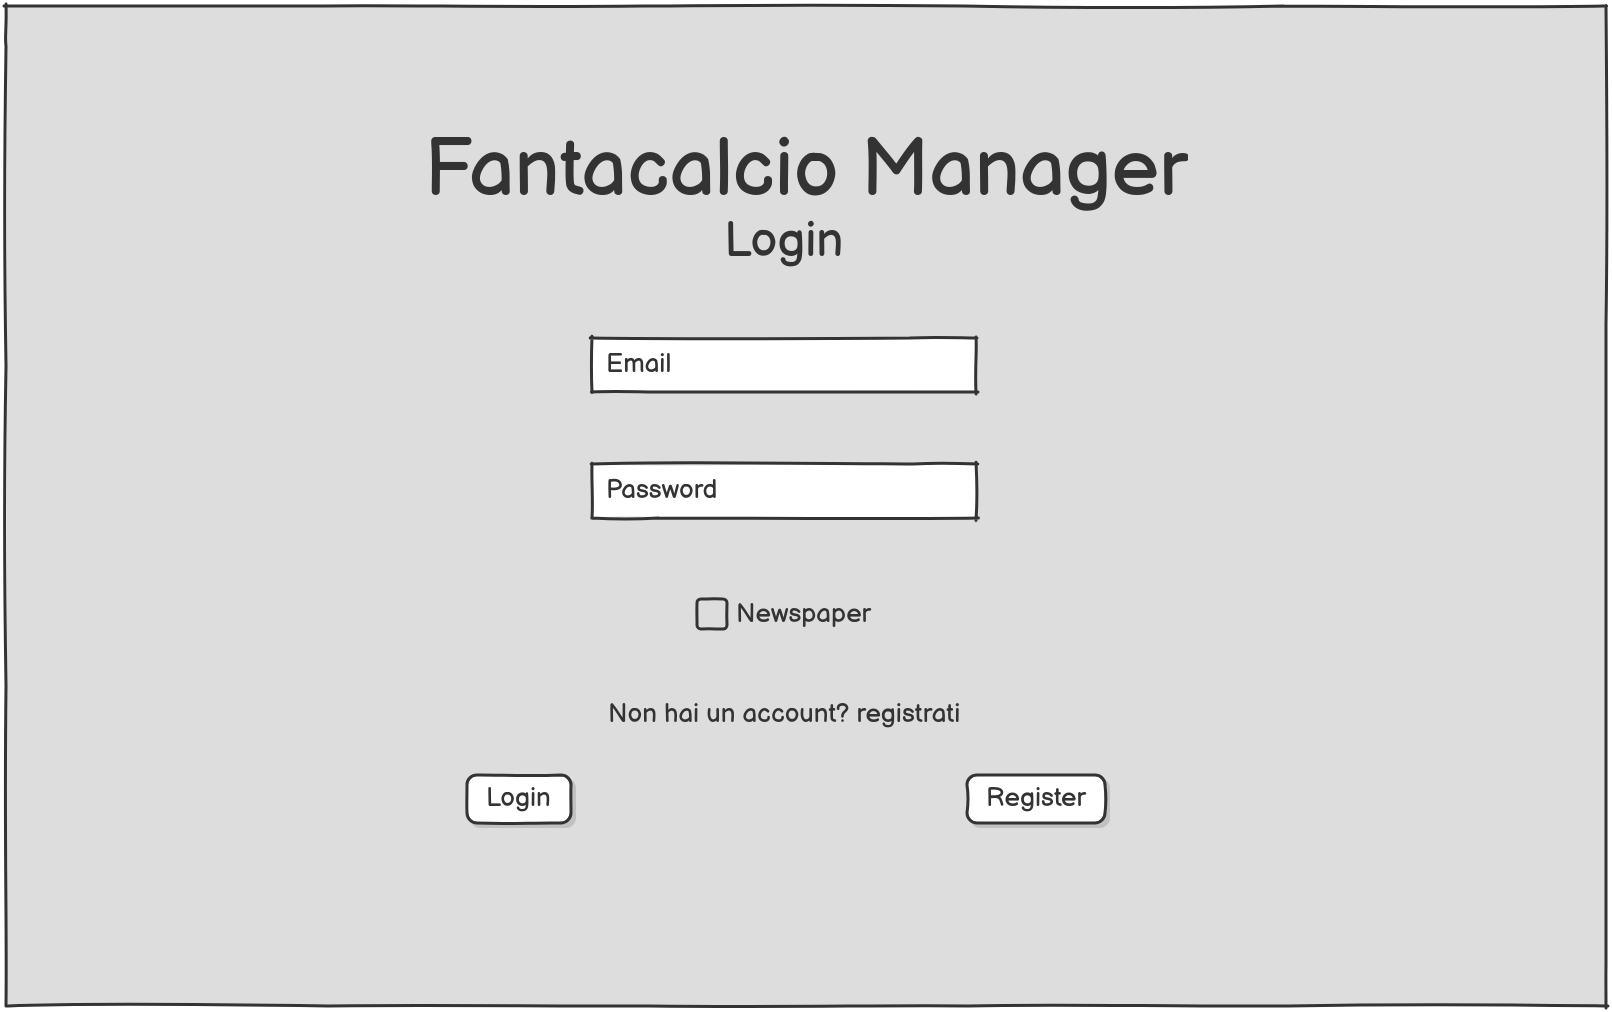
\includegraphics[width=\textwidth]{Resources/Mockups/Login.png}
        \caption{Mockup della pagina di login.}
        \label{fig:pagina_login}
    \end{subfigure}
    \hfill
    \begin{subfigure}[b]{0.49\textwidth}
        \centering
        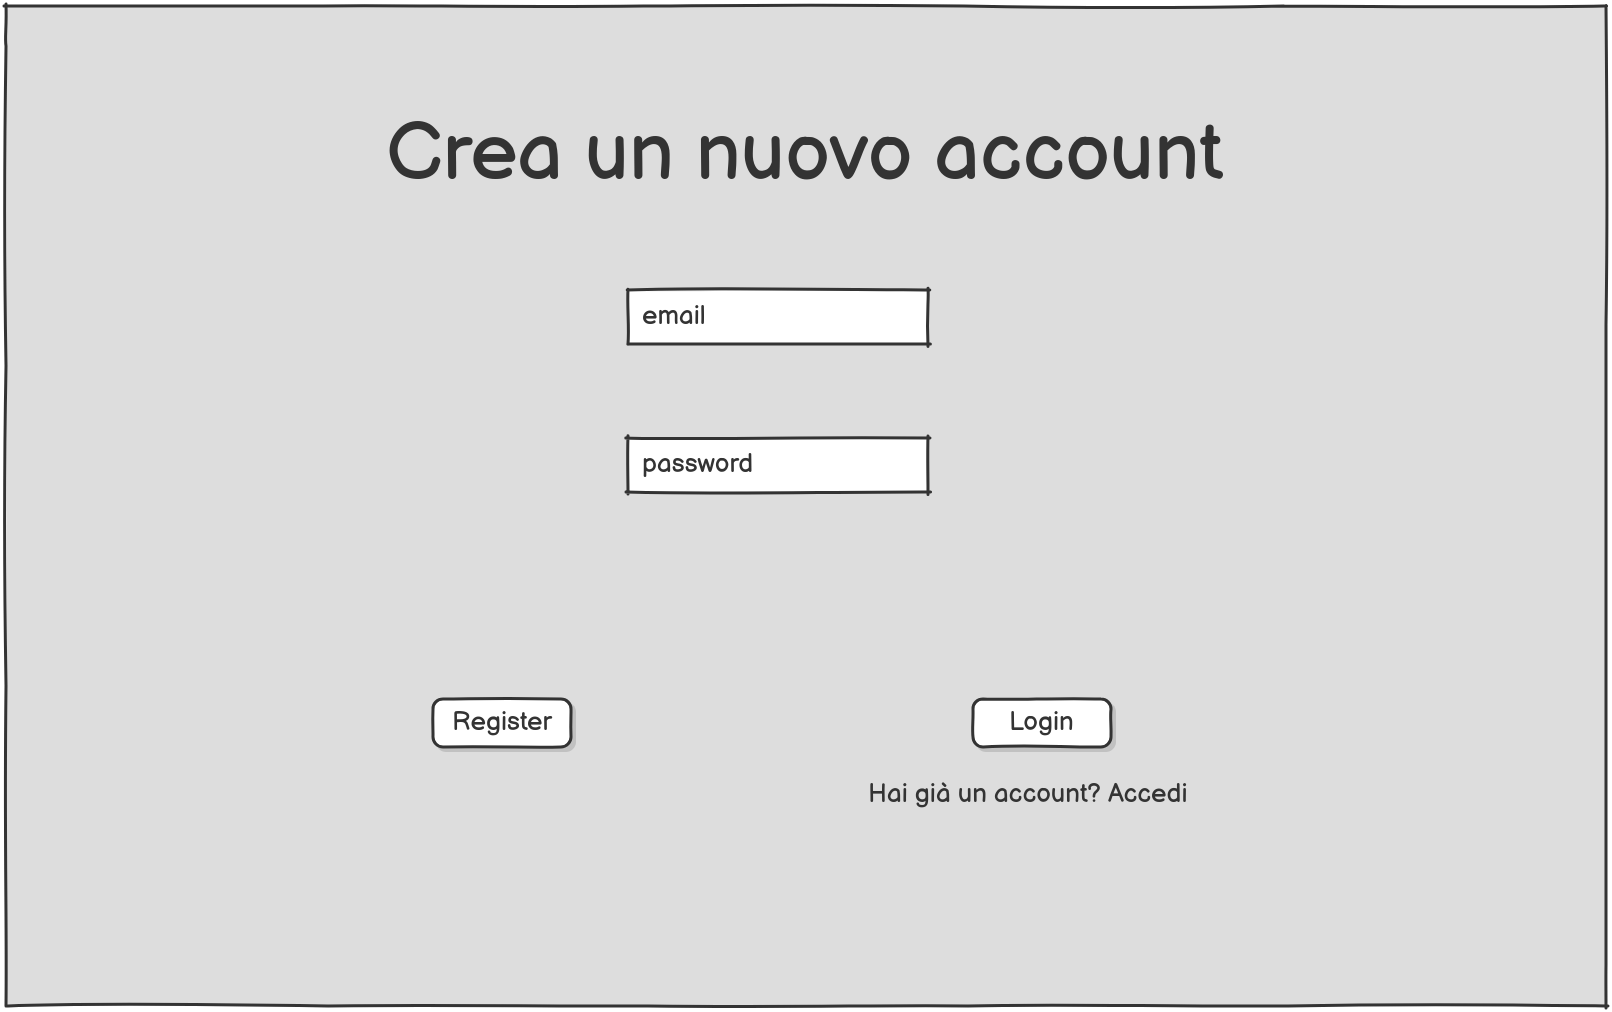
\includegraphics[width=\textwidth]{Resources/Mockups/Registrazione.png}
        \caption{Mockup della pagina di registrazione.}
        \label{fig:pagina_registrazione}
    \end{subfigure}

    % 2ª riga
    \begin{subfigure}[b]{0.49\textwidth}
        \centering
        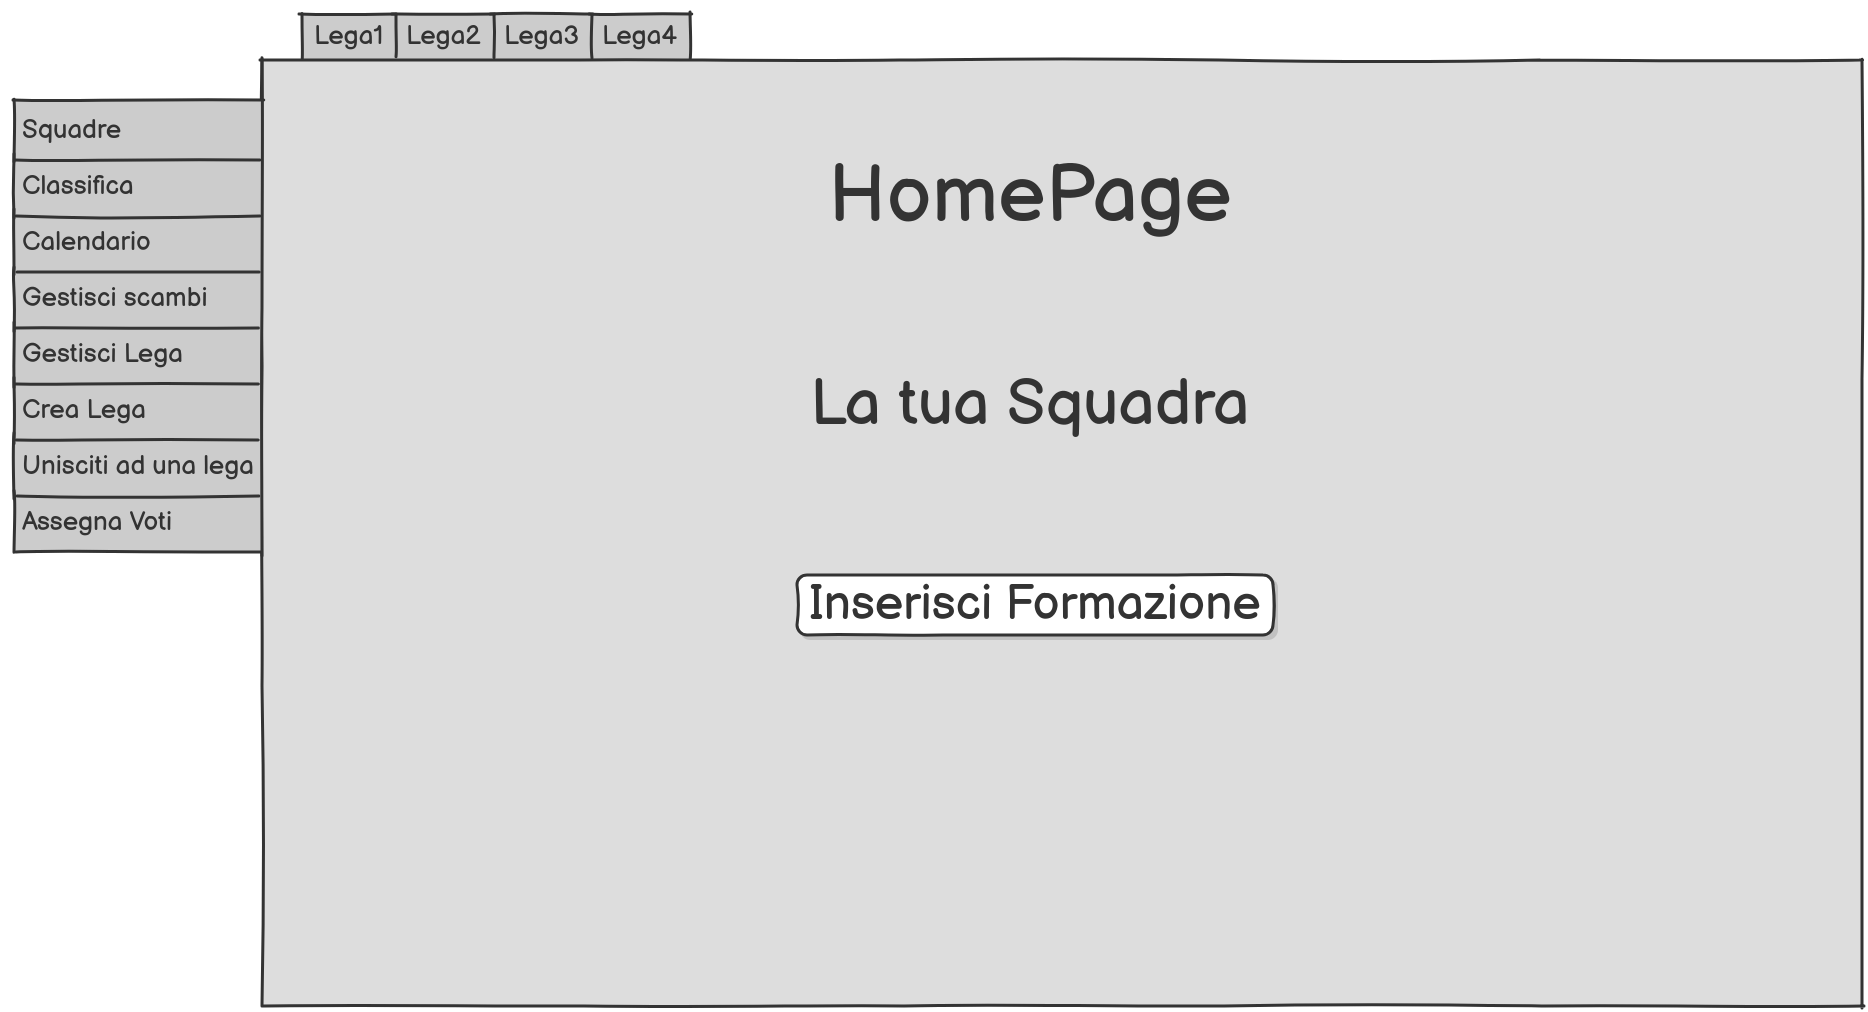
\includegraphics[width=\textwidth]{Resources/Mockups/HomePage.png}
        \caption{Mockup della homepage.}
        \label{fig:pagina_homepage}
    \end{subfigure}
    \hfill
    \begin{subfigure}[b]{0.49\textwidth}
        \centering
        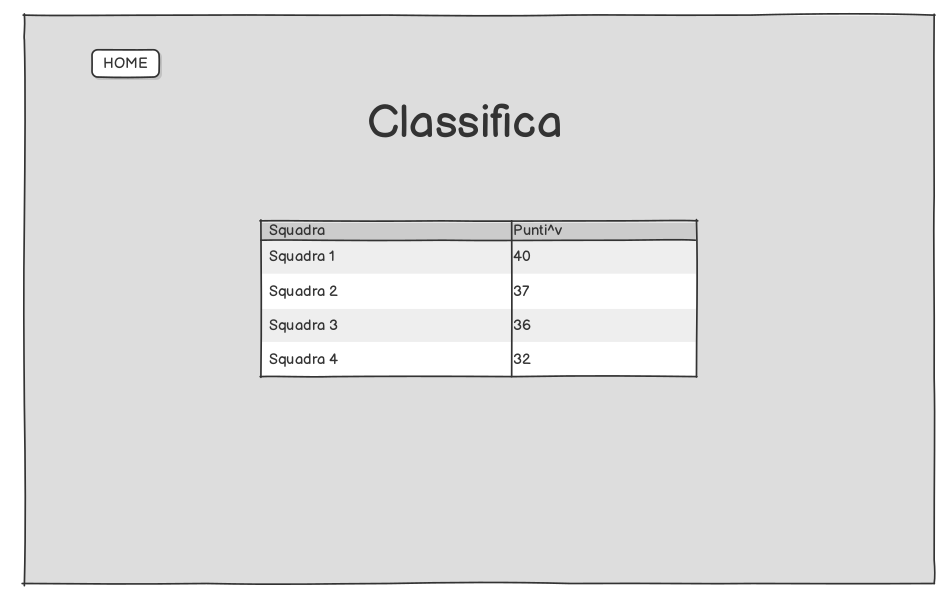
\includegraphics[width=\textwidth]{Resources/Mockups/Classifica.png}
        \caption{Mockup della classifica.}
        \label{fig:pagina_classifica}
    \end{subfigure}

    \caption{Mockup delle pagine di accesso e homepage.}
    \label{fig:mockup_parte1}
\end{figure}
\begin{figure}[H]
    \centering

    % 3ª riga
    \begin{subfigure}[b]{0.49\textwidth}
        \centering
        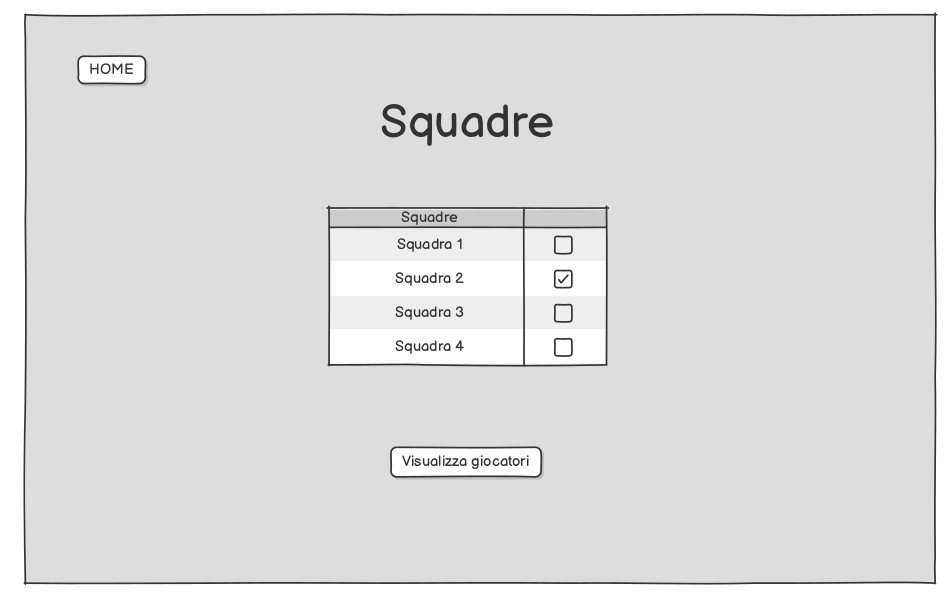
\includegraphics[width=\textwidth]{Resources/Mockups/Squadre.png}
        \caption{Mockup della pagina delle squadre.}
        \label{fig:pagina_squadre}
    \end{subfigure}
    \hfill
    \begin{subfigure}[b]{0.49\textwidth}
        \centering
        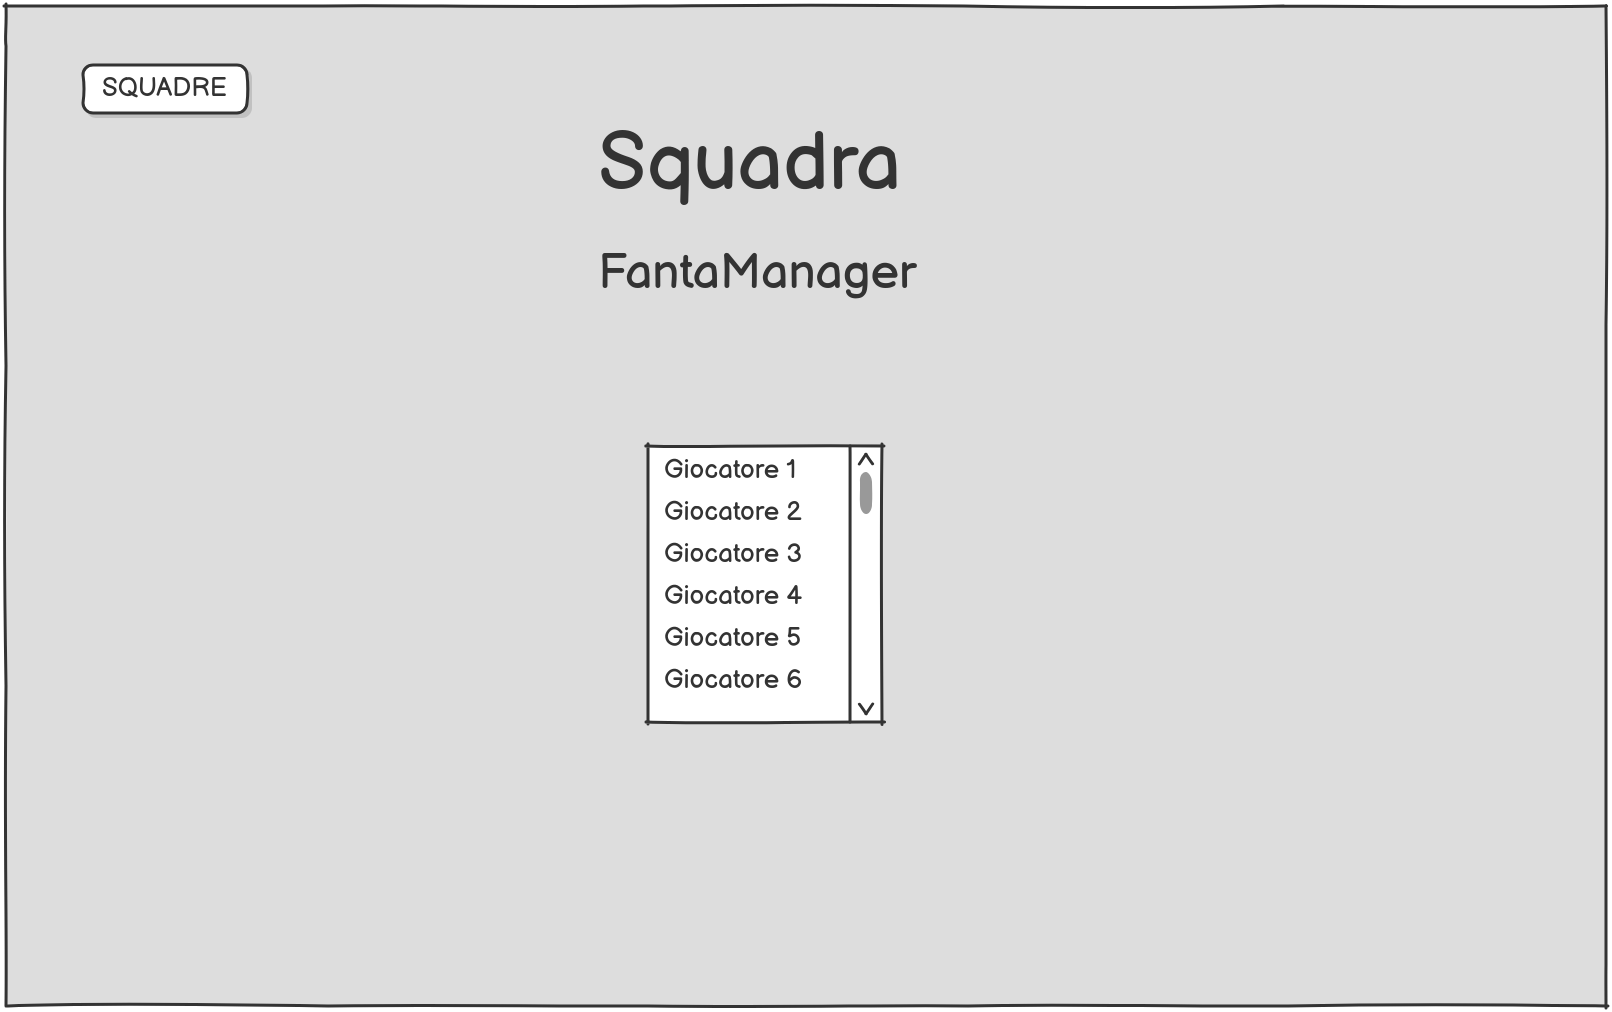
\includegraphics[width=\textwidth]{Resources/Mockups/VisualizzaSquadra.png}
        \caption{Mockup pagina di visualizzazione di un team.}
        \label{fig:pagina_visualizza_squadra}
    \end{subfigure}

    % 4ª riga
    \begin{subfigure}[b]{0.49\textwidth}
        \centering
        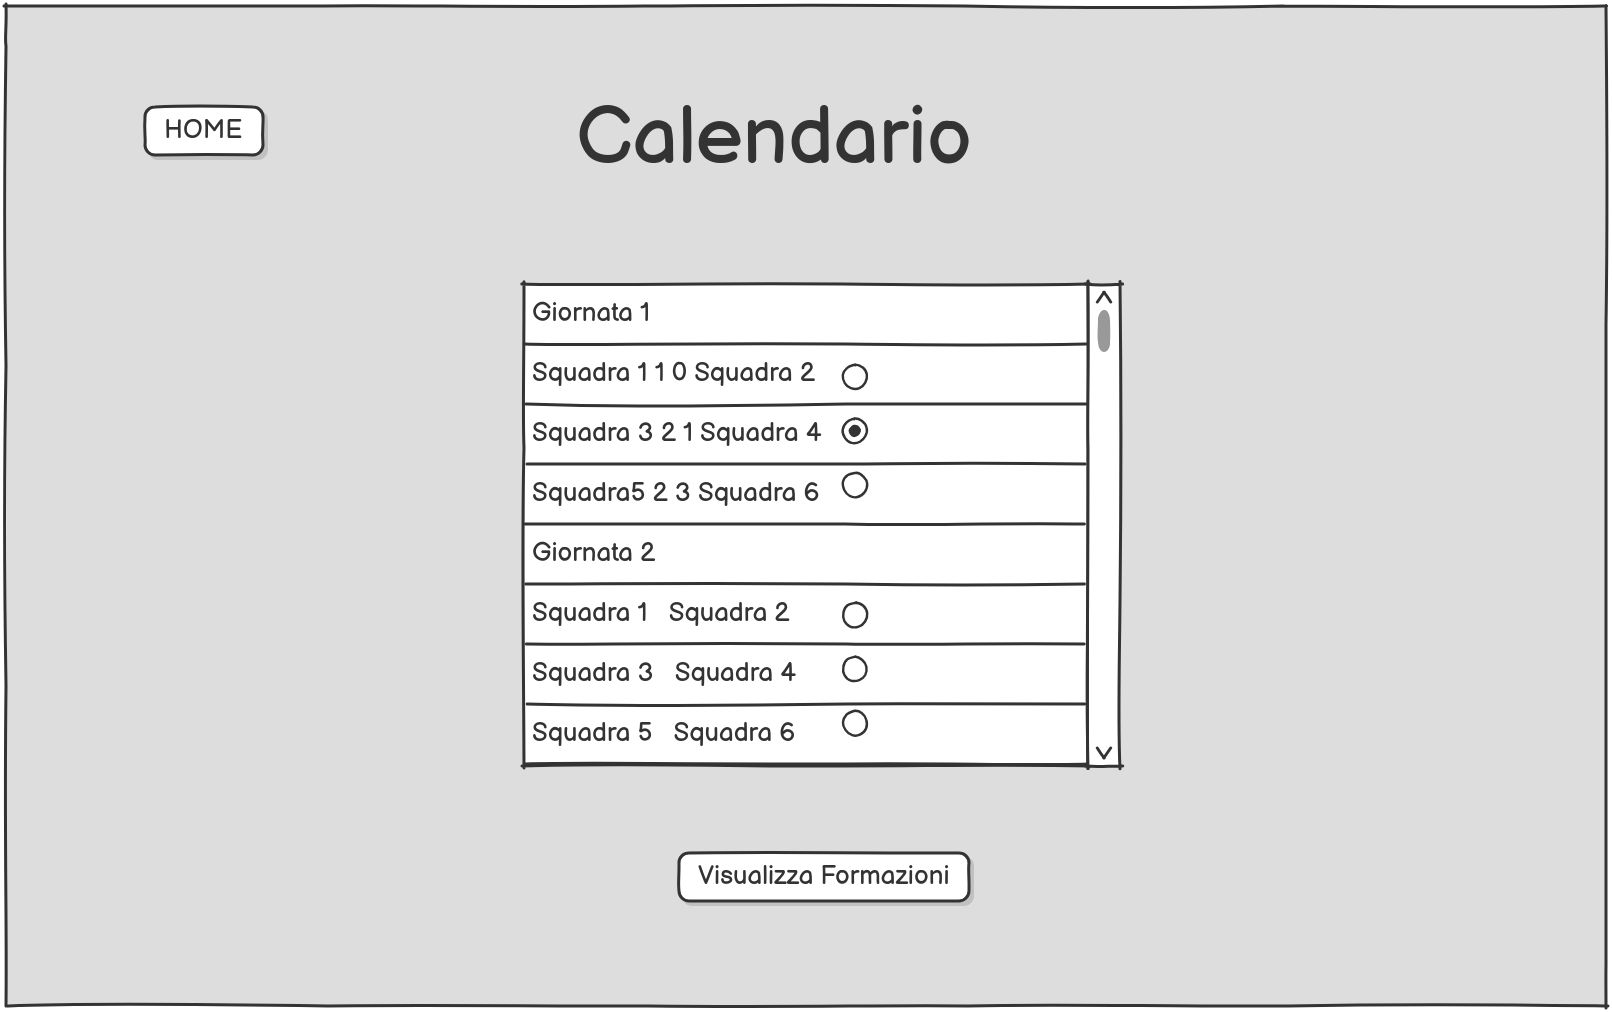
\includegraphics[width=\textwidth]{Resources/Mockups/Calendario.png}
        \caption{Mockup della pagina del calendario.}
        \label{fig:pagina_calendario}
    \end{subfigure}
    \hfill
    \begin{subfigure}[b]{0.49\textwidth}
        \centering
        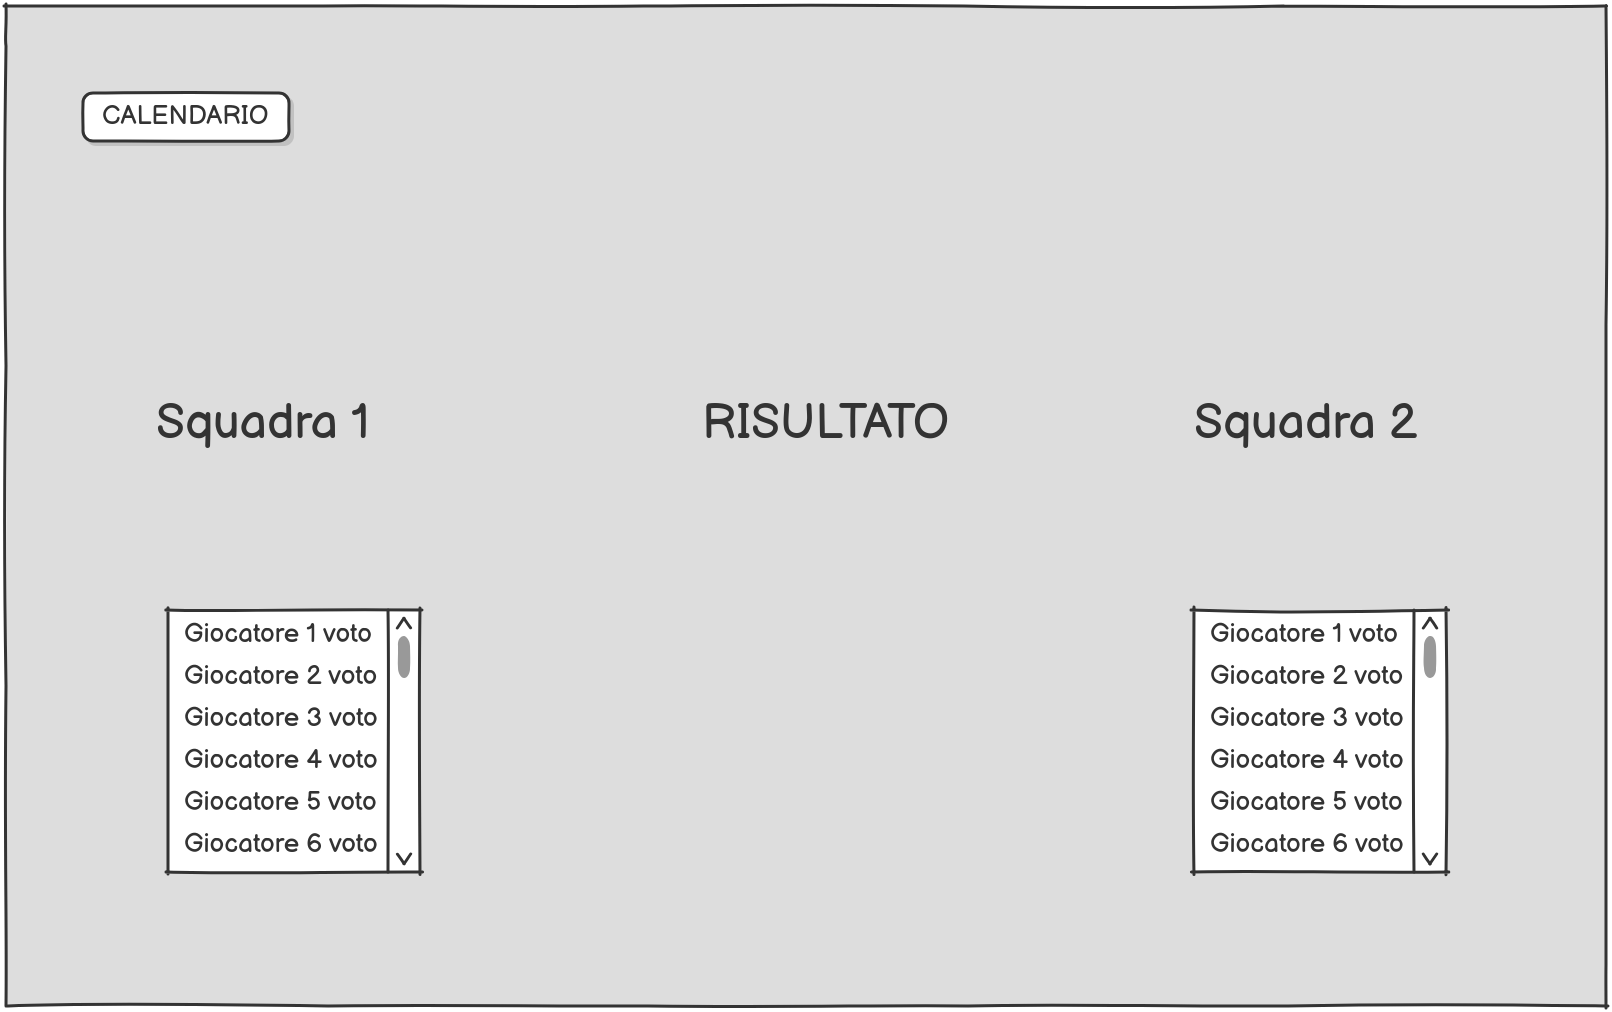
\includegraphics[width=\textwidth]{Resources/Mockups/VisualizzaMatch.png}
        \caption{Mockup pagina di visualizzazione di un match.}
        \label{fig:pagina_visualizza_match}
    \end{subfigure}

    \caption{Mockup delle pagine relative a squadre, calendario e match.}
    \label{fig:mockup_parte2}
\end{figure}
\clearpage
\begin{figure}[H]
    \centering

    % 5ª riga
    \begin{subfigure}[b]{0.49\textwidth}
        \centering
        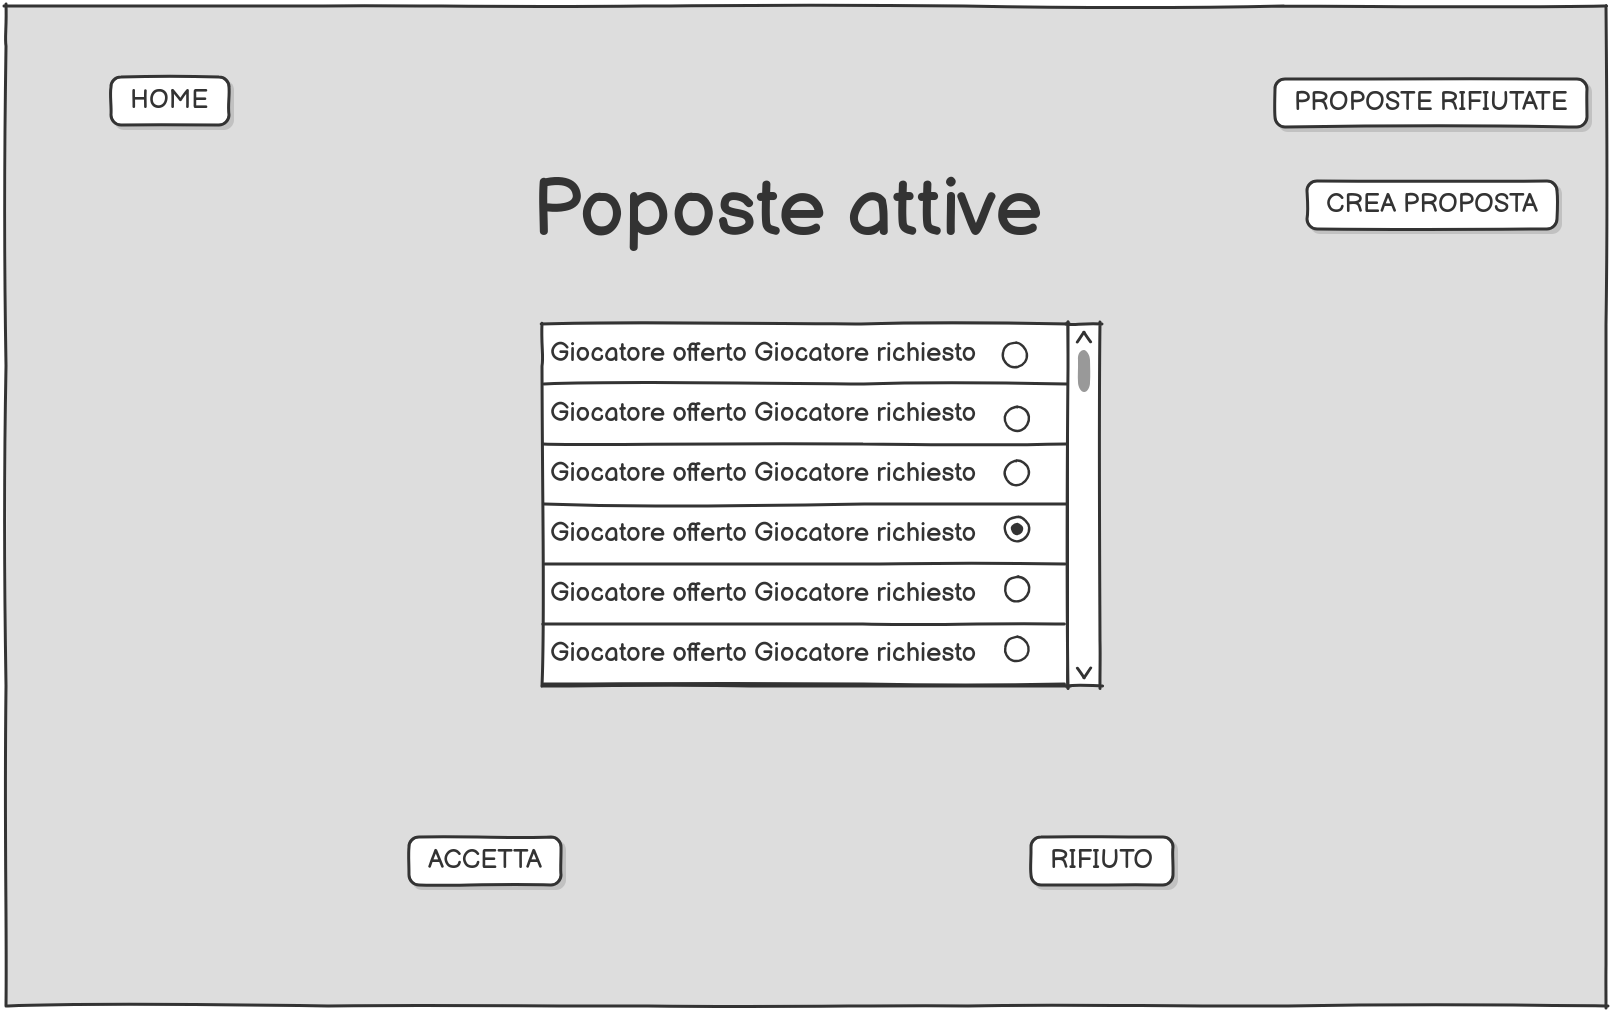
\includegraphics[width=\textwidth]{Resources/Mockups/ProposteAttive.png}
        \caption{Mockup della pagina delle proposte attive.}
        \label{fig:pagina_proposte_attive}
    \end{subfigure}
    \hfill
    \begin{subfigure}[b]{0.49\textwidth}
        \centering
        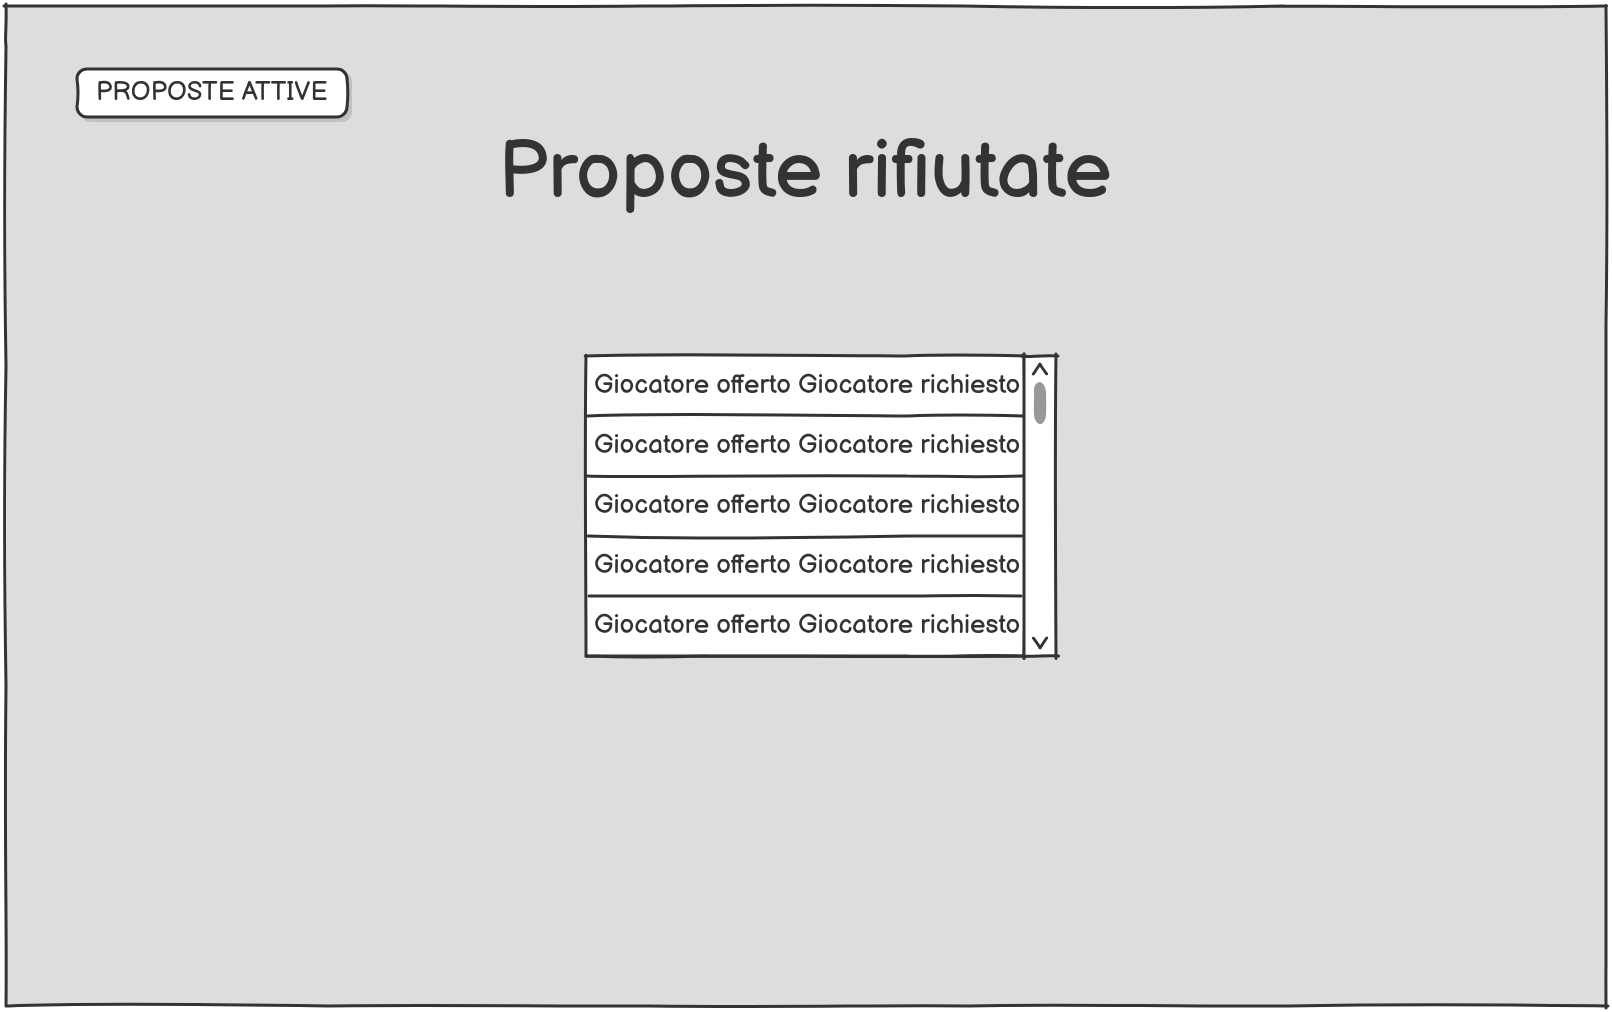
\includegraphics[width=\textwidth]{Resources/Mockups/ProposteRifiutate.png}
        \caption{Mockup della pagina delle proposte rifiutate.}
        \label{fig:pagina_proposte_rifiutate}
    \end{subfigure}

    % 6ª riga
    \begin{subfigure}[b]{0.49\textwidth}
        \centering
        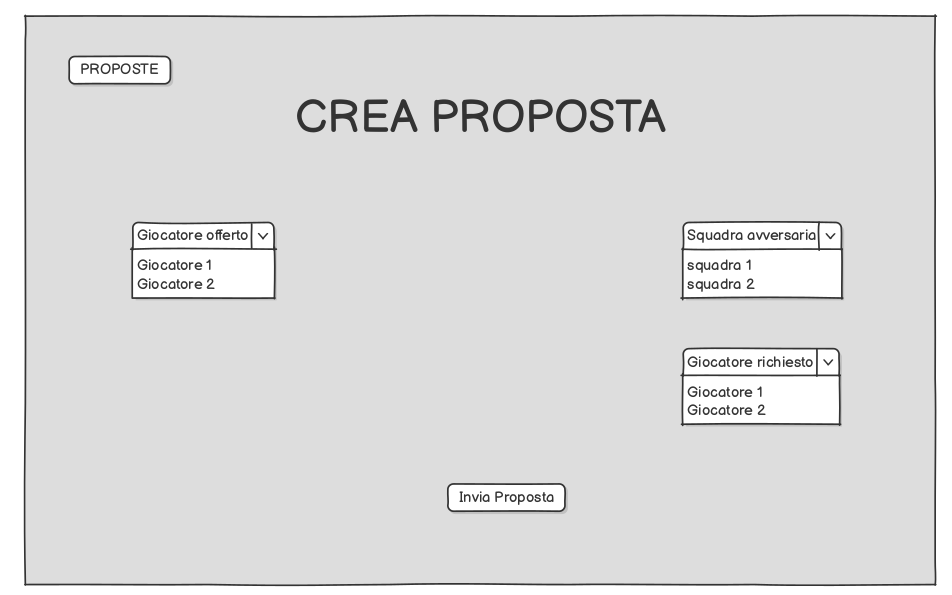
\includegraphics[width=\textwidth]{Resources/Mockups/CreaProposta.png}
        \caption{Mockup pagina per la creazione delle proposte.}
        \label{fig:pagina_crea_proposta}
    \end{subfigure}
    \hfill
    \begin{subfigure}[b]{0.49\textwidth}
        \centering
        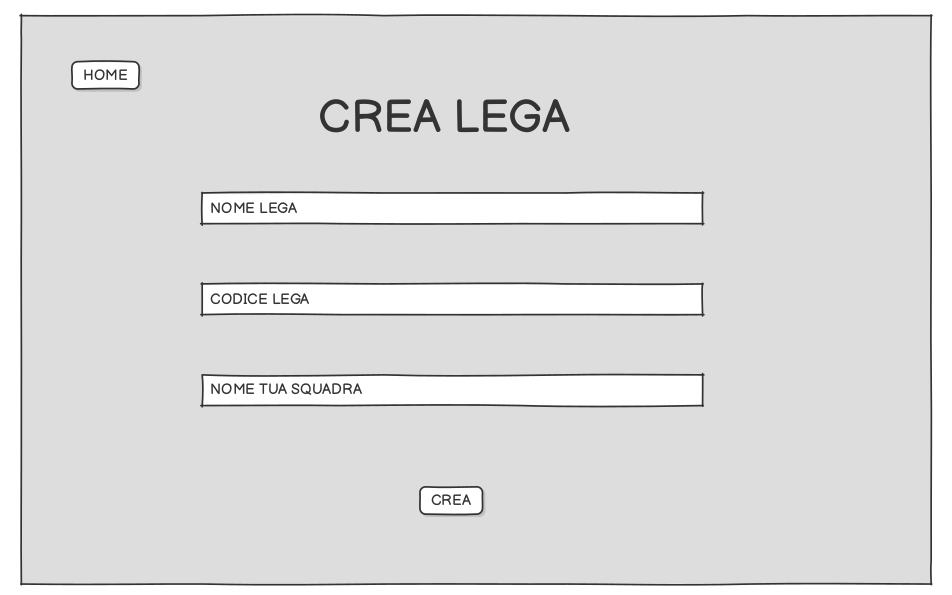
\includegraphics[width=\textwidth]{Resources/Mockups/CreaLega.png}
        \caption{Mockup della pagina di creazione di una lega.}
        \label{fig:pagina_crea_lega}
    \end{subfigure}

    \caption{Mockup delle pagine relative a proposte e creazione di leghe.}
    \label{fig:mockup_parte3}
\end{figure}
\begin{figure}[H]
    \centering

    % 7ª riga
    \begin{subfigure}[b]{0.49\textwidth}
        \centering
        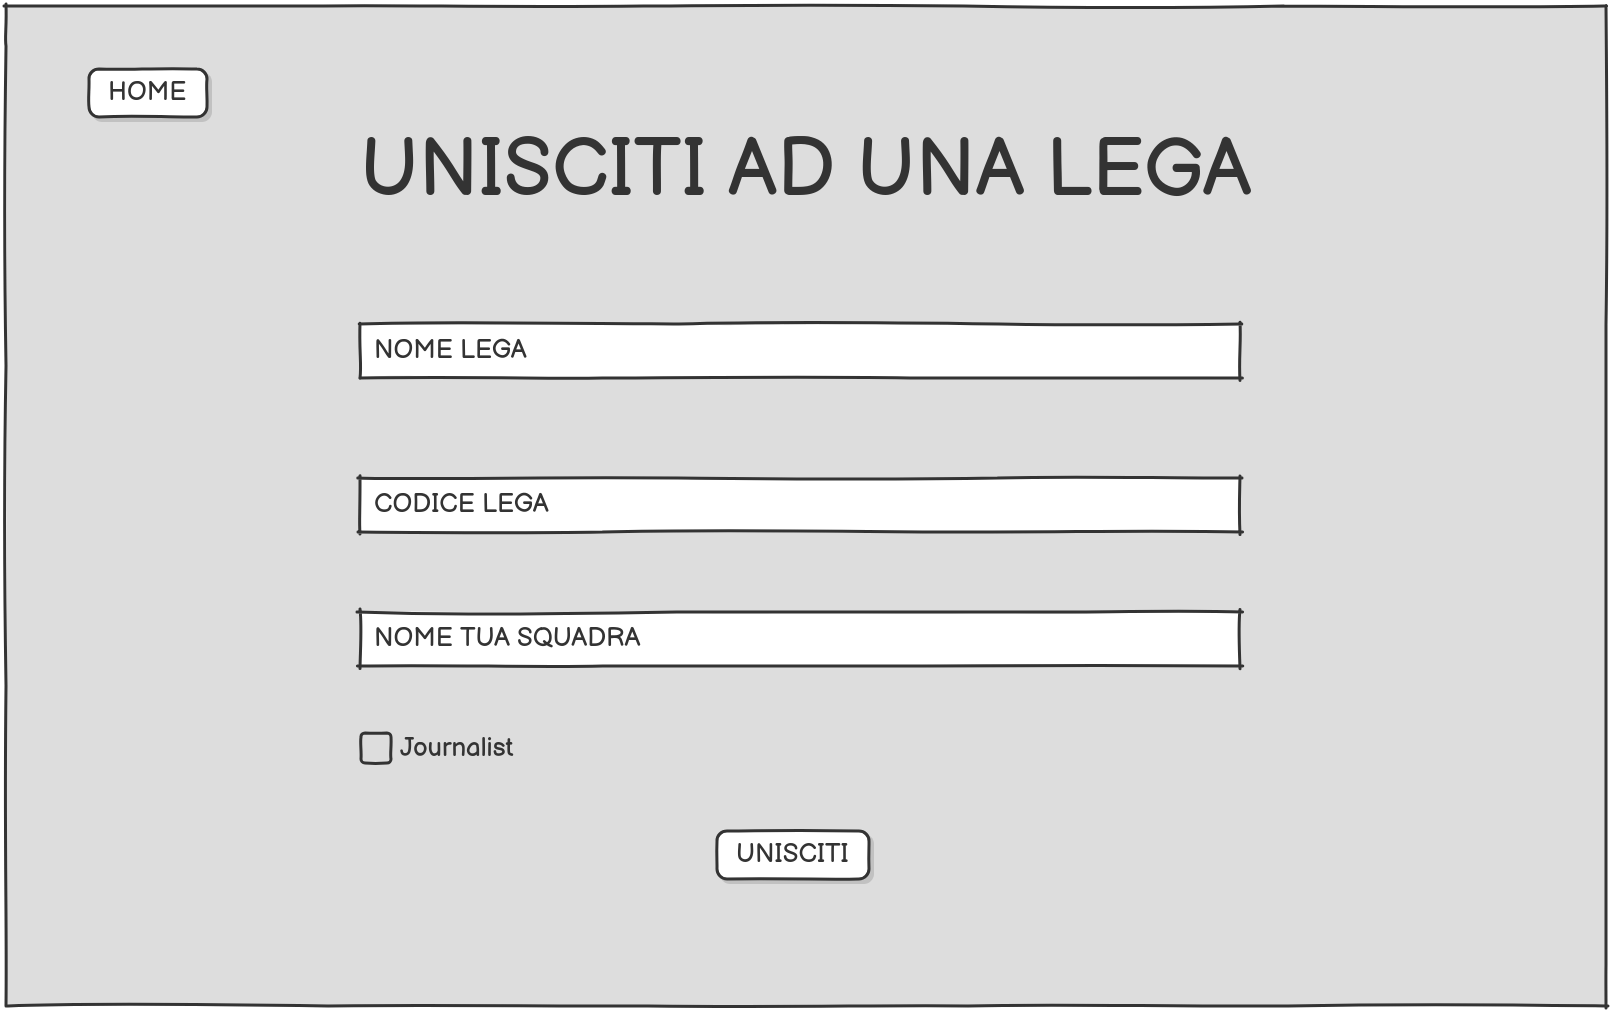
\includegraphics[width=\textwidth]{Resources/Mockups/UniscitiAdUnaLega.png}
        \caption{Mockup della pagina per l'adesione a una lega.}
        \label{fig:pagina_unisciti_lega}
    \end{subfigure}
    \hfill
    \begin{subfigure}[b]{0.49\textwidth}
        \centering
        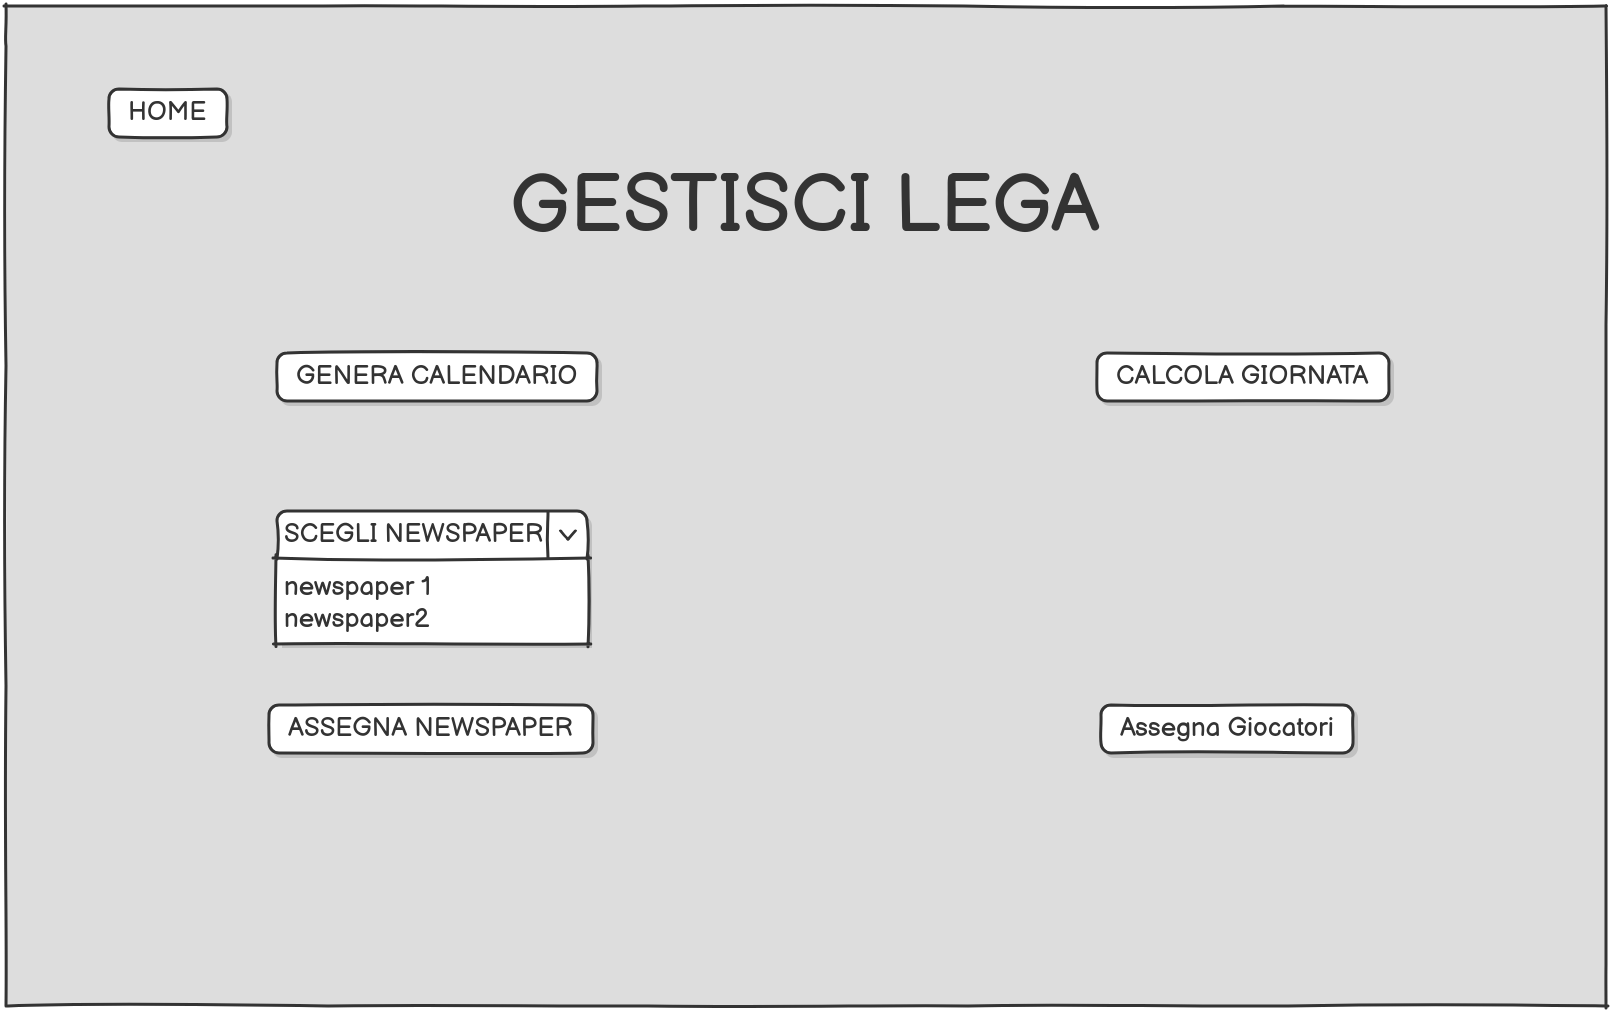
\includegraphics[width=\textwidth]{Resources/Mockups/GestisciLega.png}
        \caption{Mockup della pagina per la gestione della lega.}
        \label{fig:pagina_gestisci_lega}
    \end{subfigure}

    % 8ª riga
    \begin{subfigure}[b]{0.49\textwidth}
        \centering
        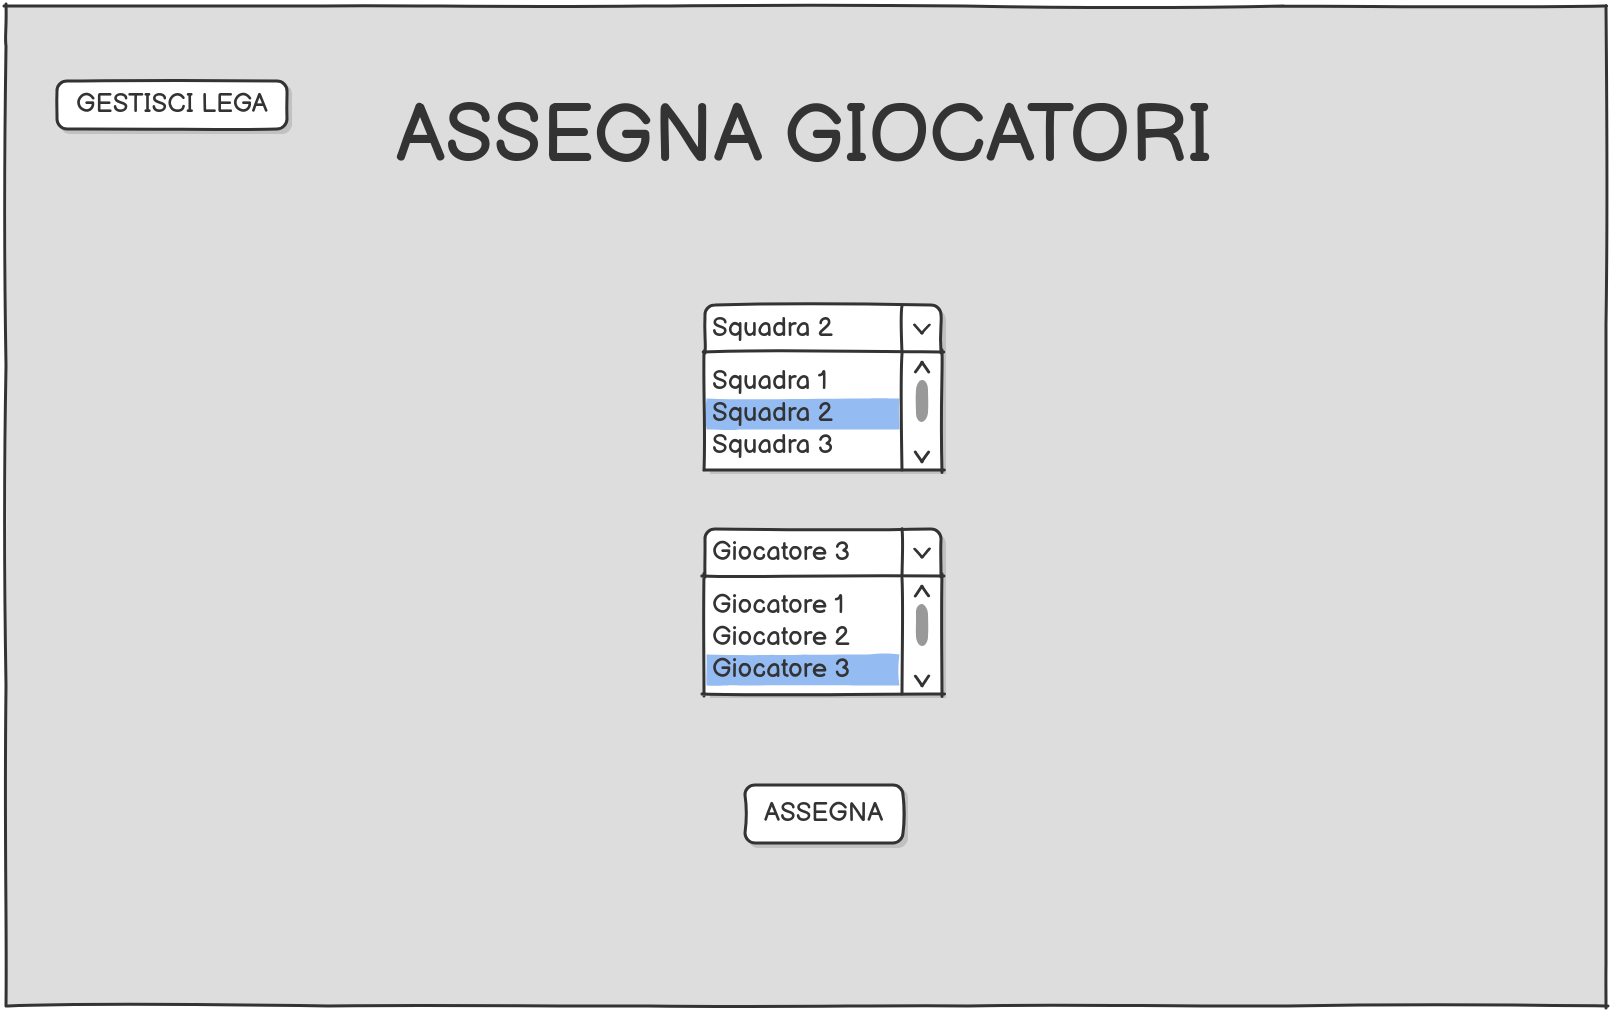
\includegraphics[width=\textwidth]{Resources/Mockups/AssegnaGiocatori.png}
        \caption{Mockup pagina assegnazione dei giocatori ai team.}
        \label{fig:pagina_assegna_giocatori}
    \end{subfigure}
    \hfill
    \begin{subfigure}[b]{0.49\textwidth}
        \centering
        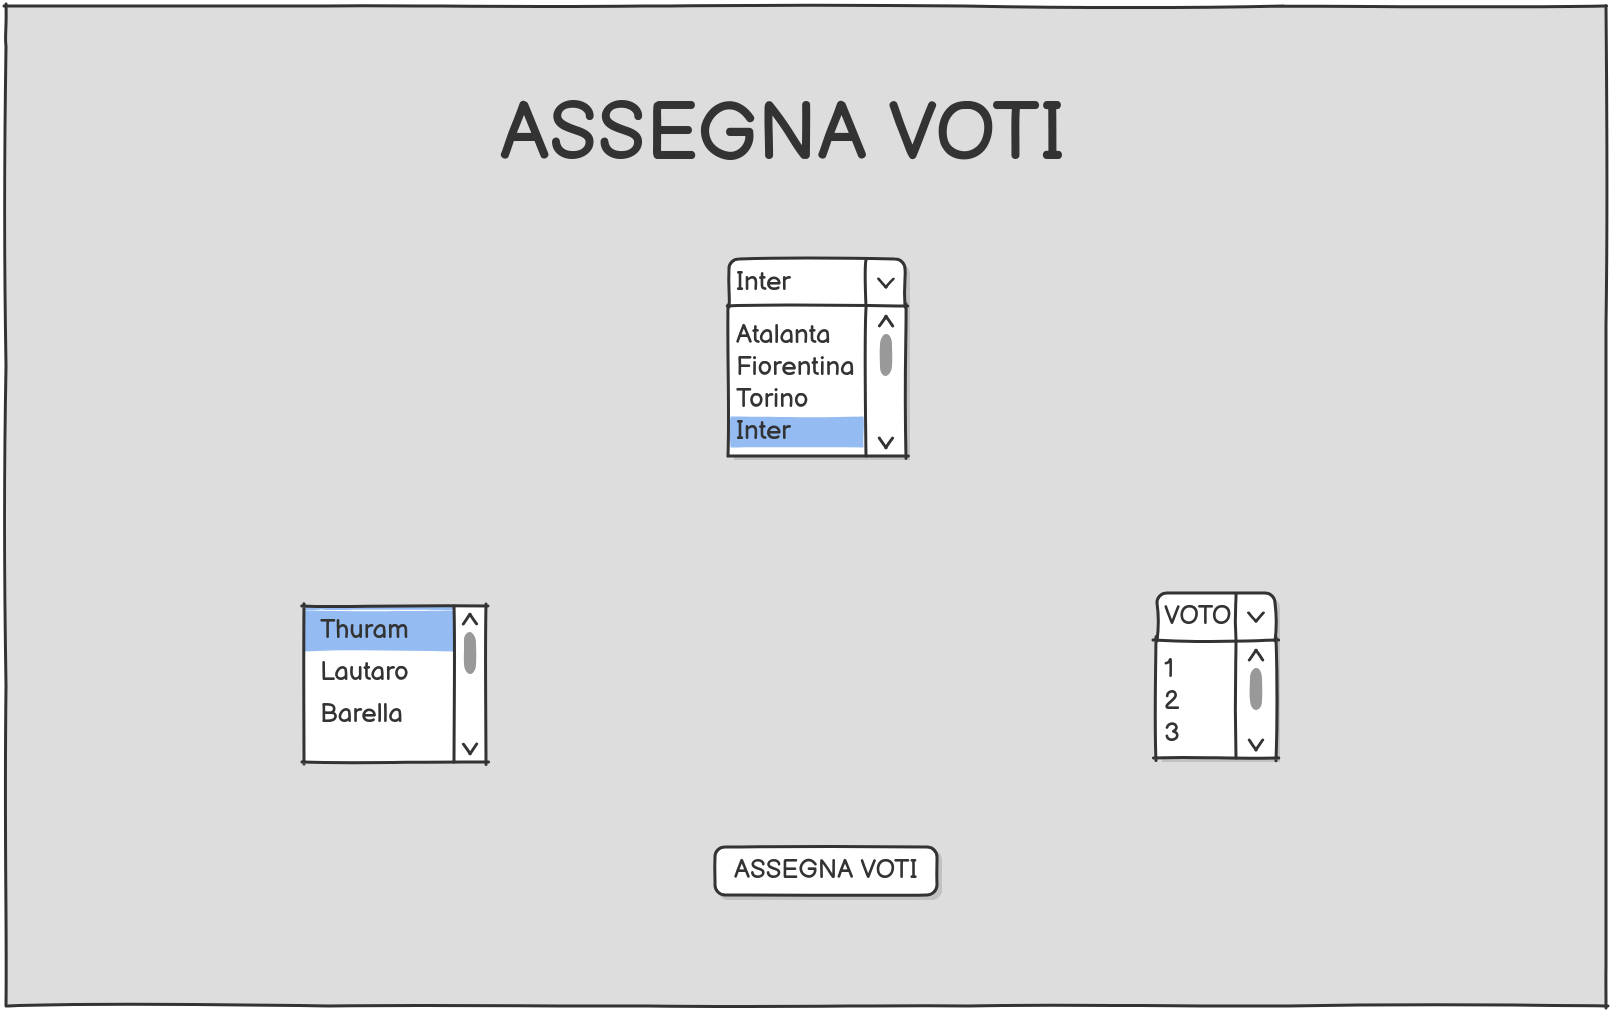
\includegraphics[width=\textwidth]{Resources/Mockups/AssegnaVoti.png}
        \caption{Mockup della pagina per l'assegnazione dei voti.}
        \label{fig:pagina_assegna_voti}
    \end{subfigure}

    \caption{Mockup delle pagine di gestione delle leghe e assegnazioni.}
    \label{fig:mockup_parte4}
\end{figure}
